\section{Super-Imposing Images}
Super-imposed images look strange if they have different orientations and translations. In fitting an image in a specific location of a background, it is crucial to ensure the images are matching properly.  This can be performed by finding homographic transformation between two images and transforming one image into the other domain before image stitching.
\par
The following implementation matches four corners of two billboards with two posters shown next to them(\ref{ps}).  Although the matching seems to have better performance(\ref{rst_1}) it required some fine-tuning along the way. It is because four matches alone are not sufficient enough to find an exact homographic transformation.

\begin{figure}[h]
    \begin{center}
        \begin{minipage}{.65\textwidth}
            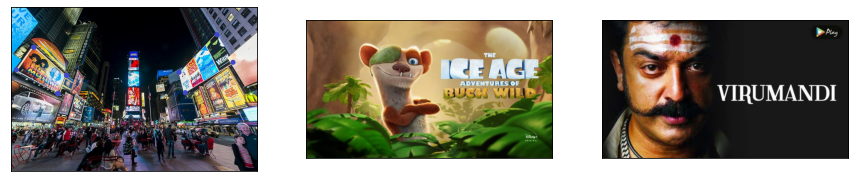
\includegraphics[width=.95\columnwidth]{q2_1}
            \caption{Billboards and Posters}
            \label{ps}
        \end{minipage}
        \begin{minipage}{.65\textwidth}
            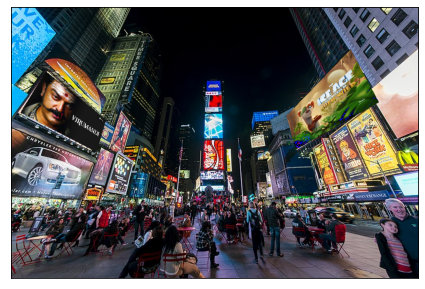
\includegraphics[width=.95\columnwidth]{q2_2}
            \caption{Overlayed Image}
            \label{rst_1}
        \end{minipage}
    \end{center}
\end{figure}


\section{SIFT Feature Matching}
Sift descriptor divides the image into $4\times 4$ sub-patches. Histograms are developed based on the data extracted from each patch using the orientation calculated and normalized to eight discrete levels. These are concatenated to form a feature vector of each feature. Through filtering and matching these feature vectors SIFT achieves robust matchings between points regardless of the variations. Top matches extracted between \textit{im1.ppm} and \textit{im5.ppm} of the Graffiti  images using SIFT is as follows:
\begin{figure}[h]
    \begin{center}
        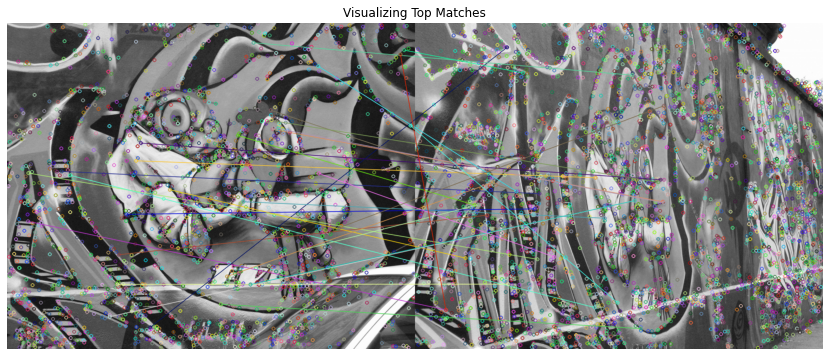
\includegraphics[width=.75\textwidth]{sift}
    \end{center}
\end{figure}